\subsection{Organisation d'une application basée sur une telle architecture}
Par opposition à une architecture du type 3 tiers, dont les services permettant d'accéder aux données se confondent avec ceux qui vont agir sur ces même données, l'architecture CQRS sépare volontairement les composants requêtant les données de ceux qui les modifient.
Une telle séparation facilite l'organisation de l'application puisque des composants différents sont utilisés pour des actions différentes.
On peut ainsi découper l'architecture du modèle CQRS en différente couches.

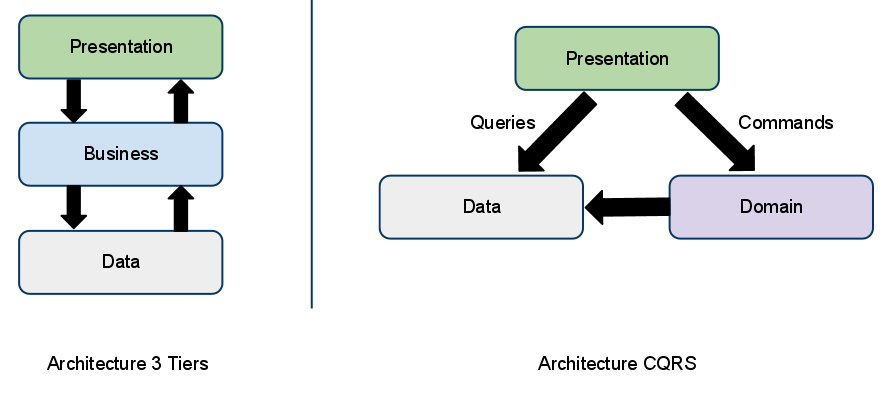
\includegraphics[scale=0.5]{Figures/Chapter3/architecture/tiersvscqrs.png}

%-------------------------------------------------------------------------
\subsubsection{La couche de modification des données: Command}
\label{subs:La couche de modification des données: Command}
\paragraph{}
Cette couche concentre toutes les modifications des données, qu'il s'agisse de création, de suppression ou de mise à jour.
Une commande représente une action destinée à être exécutée, une intention, et n'est pas une simple demande d'altération de donnée.
Généralement, une commande est représentée comme un appel de méthode encapsulée dans un objet; elle porte un nom explicite et ses champs contiennent les différents paramètres de l'action.
Dans le cas de l'espace recruteur du site Cadremploi.fr, les commandes ont pour but d'enregistrer les altérations effectuées par les événements côté client, et on retrouve des commandes nommées 'ModifierDescriptionPosteCommand' ou 'PayerOffreCommand' par exemple.
De tels noms sont ainsi très expressifs et permettent de clarifier la cause de la modification des données.

%-------------------------------------------------------------------------
\subsubsection{La couche de lecture des données: Query}
\label{subs:La couche de lecture des données: Query}
La partie Query de ce modèle se base sur le fait que les objets du modèle sont volumineux et qu'il est possible de s'en passer.
Cette couche fonctionne ainsi uniquement en lecture seule, aucune modification n'est apportée aux données.
En effet le besoin représenté ici est celui d'une lecture dans un cas d'utilisation bien précis, l'objectif est d'aller extrêmement vite.
Le pattern Query consiste alors à exécuter une requête précise en base et de restituer un objet de type Data Transfer Object (DTO) concis qui pourra être utilisé directement.
Cela signifie que les contrôles sont réduits au minimum et que les DTOs utilisés sont des objets représentant exactement et uniquement le besoin en lecture, généralement des besoins IHM.
Cette méthode permet de récupérer seulement les données dont on a besoin en une fois, en se passant ainsi de parcourir plusieurs tables à travers desquelles les données seraient éparpillées.

%-------------------------------------------------------------------------
\subsubsection{Le domaine}
\label{subs:Le domaine}
Le domaine est la zone où est concentré toute la connaissance métier de l'application.
C'est de là que chaque commande est analysée et qu'il est décidé si l'on donne suite à chacune d'entre elle.
On y trouve ainsi les différents objets permettant de pratiquer les contrôles nécessaires entre autre.
